\chapter{Software Independence}

A good practice is to write as much software as independent as possible from architectures and platforms
to maximize software \textbf{portability} and \textbf{reusability}.

It's impossible to make everything independent as firmware layers still intersct with hardware and
Assembly code is archiecture dependent as it depends on that hardware's IS.

\begin{figure}[H]
    \centering
    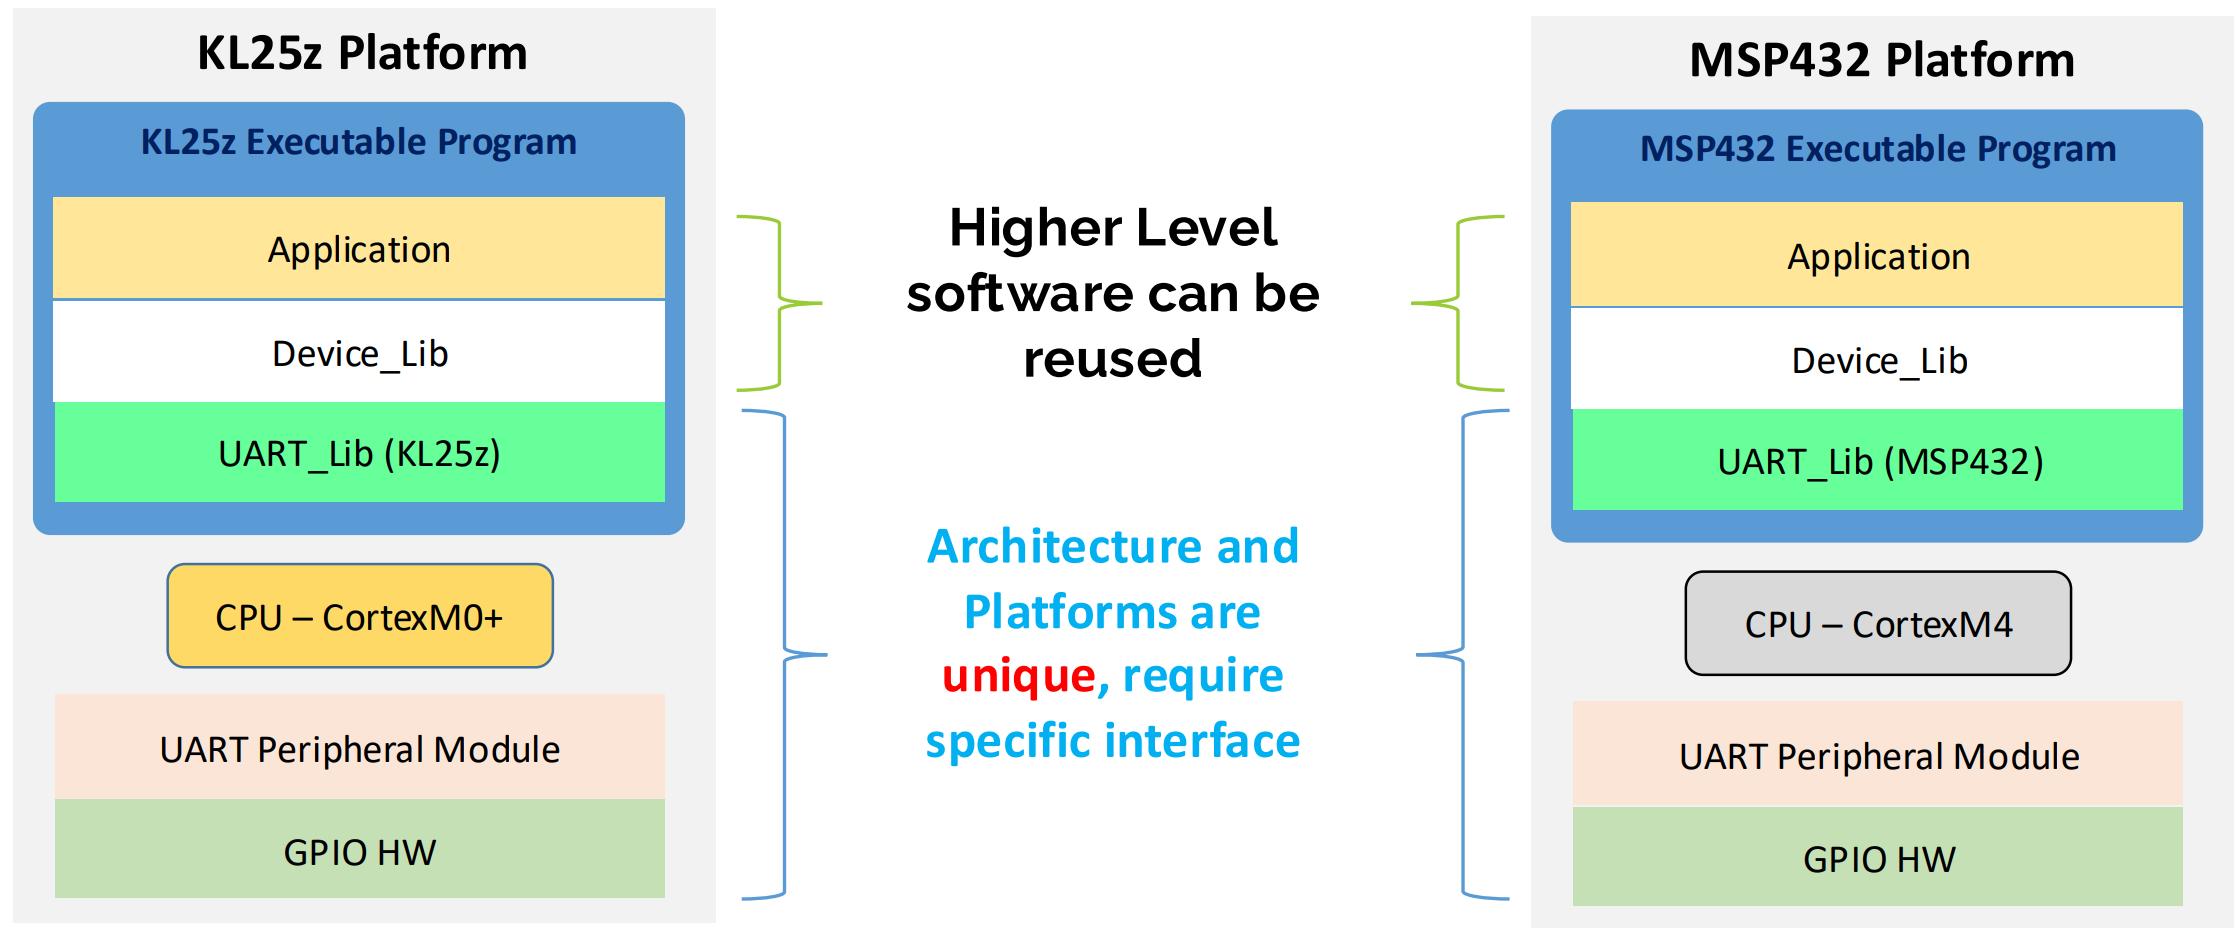
\includegraphics[width=0.75\linewidth]{img/image81.png}
\end{figure}

\section{Binary Interfaces}
The Embedded Application Binary Interface (EABI) is a set of conventions and standards to provide
guidelines for:


\begin{itemize}
    \item how functions are called
    \item how data is organized in memory
    \item how exceptions are handled in embedded applications.
\end{itemize}

Binary interfaces specify details of how the executable must run on this architecture (done by compilers in
most cases).

In architecture terms, an instruction is a fundamental unit of work or operation (arithmetic, logical, program
flow control, load/store), while a word is a fundamental operand size for each operation.

\paragraph{Instruction Sizes:} Instruction size can vary between instruction sets (like ARMv6-M and Thumb-2, for example).
\paragraph{}
Instruction – Fundamental unit of work or operation (Arithmetic, Logical, Program Flow Control, Load/Store)

Word – fundamental operand size for each operation


\paragraph{Standard Integer Sizes: }Variable length types can cause portability issues, we want \textbf{portable data types}. Explicitly defined types that specify storage and design are defined in the \verb|stdint.h| header file.


\begin{lstlisting}[language=c++]

    #ifndef __STDINT_H__
    #define __STDINT_H__
    
    /* 8-bit signed/unsigned Integers */
    typedef signed char int8_t;
    typedef unsigned char uint8_t;
    
    /* 16-bit signed/unsigned Integers */
    typedef signed short int int16_t;
    typedef unsigned short int uint16_t;
    
    /* 32-bit signed/unsigned Integers */
    typedef signed long int int32_t;
    typedef unsigned long int uint32_t;
    
    /* 64-bit signed/unsigned Integers */
    typedef signed long long int int64_t;
    typedef unsigned long long int uint64_t;
    
    #endif /* __STDINT_H__ */
\end{lstlisting}

\section{Pointer Types}

All Pointers are the same length. This because pointer hold addresses in memory of 32-bit.

We need to cast in order to obtain the data inside the memory.

\begin{equation*}
    sizeof(uint8_t*) = sizeof(int16_t*) = sizeof(uint32_t*) = sizeof(float*) = \text{32-Bits!}
\end{equation*}

\begin{lstlisting}[language=c++]

    uint8_t * ptr1 = (uint8_t *) 0x00;
    uint16_t * ptr2 = (uint16_t *) 0x04;
    uint32_t * ptr3 = (uint32_t *) 0x08;
    float * ptr4 = (float *) 0x0C;
\end{lstlisting}

\begin{equation*}
    sizeof(ptr1) = sizeof(ptr2) = sizeof(ptr3) = sizeof(ptr4) = \text{32-Bits!}
\end{equation*}
\begin{equation*}
    sizeof(*ptr1) \ne sizeof(*ptr2)  \ne sizeof(*ptr3)  \ne sizeof(*ptr4)
\end{equation*}

\subsection{NULL Pointers}

In embedded platforms it is always the device (no OS, no other software) that uses pointers carefully.

Null Pointers point to nothing, dereferencing a NULL Pointer can cause an \textbf{exception}.

\section{Data alignment}

\begin{figure}[H]
    \centering
    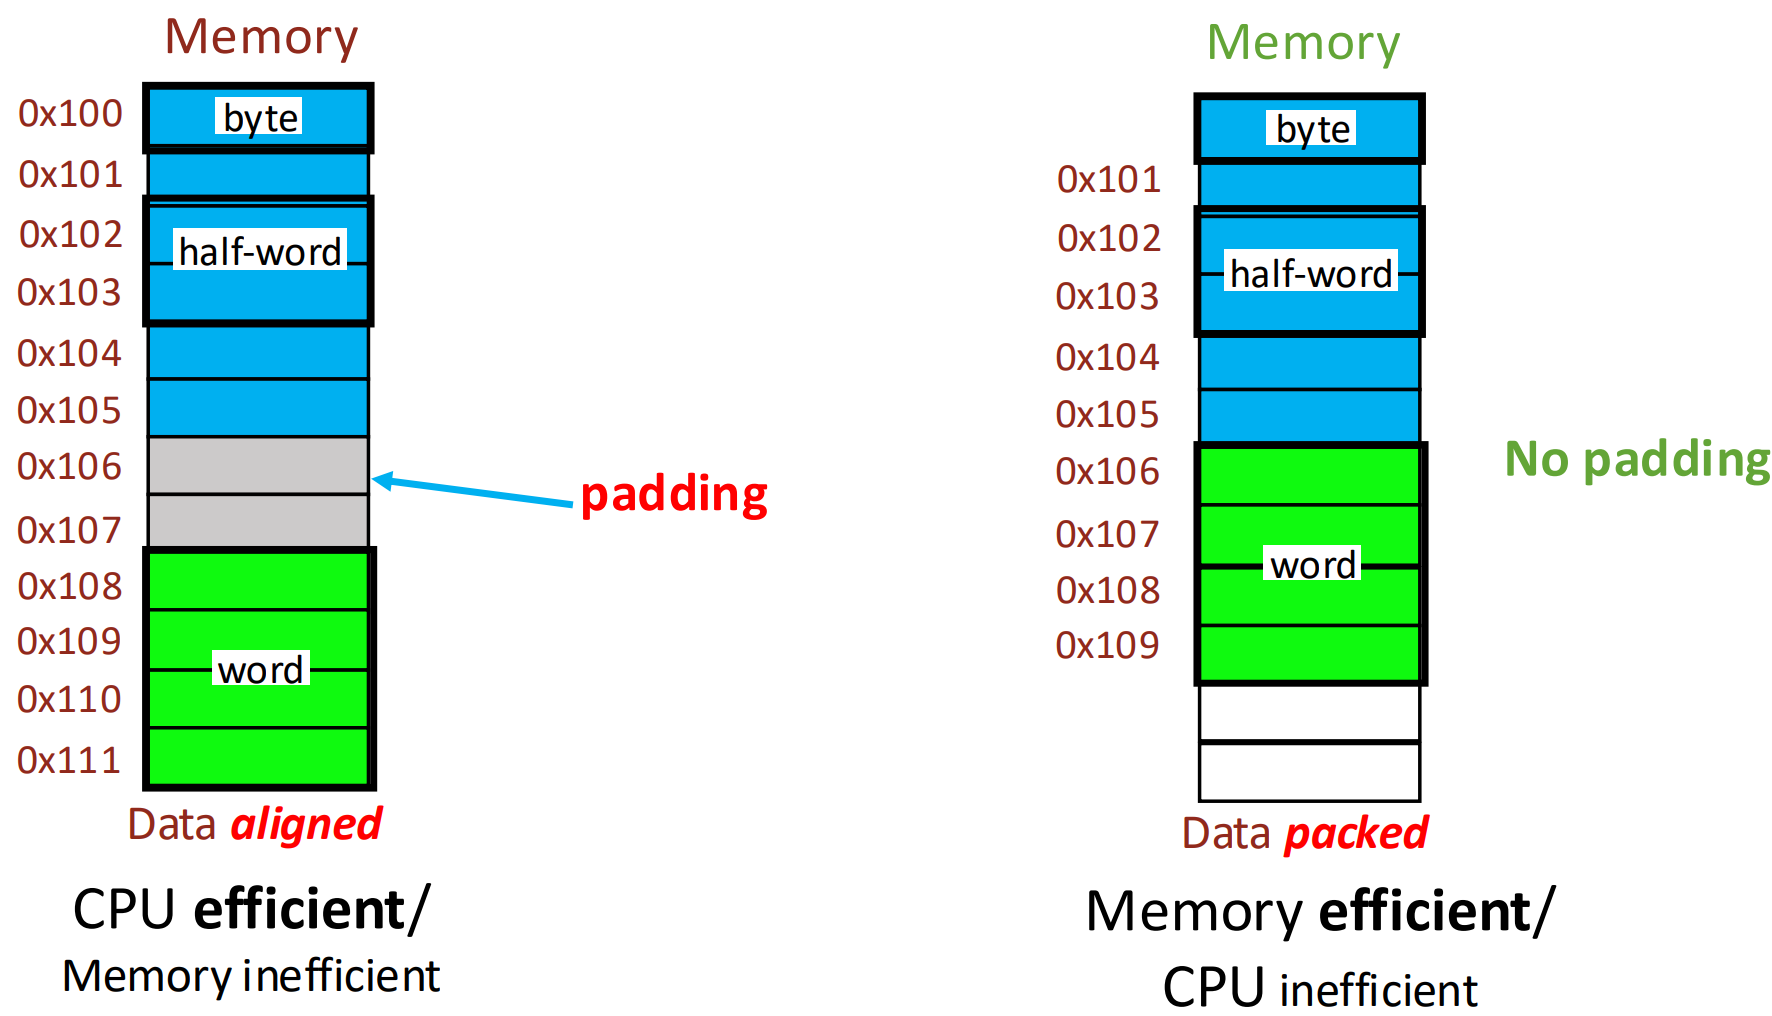
\includegraphics[width=0.75\linewidth]{img/image82.png}
\end{figure}


\textbf{Load/store data occurs only at aligned addresses in memory.}

\subsection{How to control alignment of data in memory}
We use a compiler attribute which changes based on the compiler.


\begin{lstlisting}[language=c++]

    struct struct_name {
        int8_t var1 int8_t var1 __attribute__ ((aligned(4)));
        int32_t var2;
        int8_t var3;
    } __attribute__ ((packed)); //if not appear default is aligned:  __attribute__ ((aligned));
\end{lstlisting}

In this case, since it's packed, the size of the structure will be 6 bytes rather than 12 bytes when data is
aligned/padded. It will be less efficient for the CPU, however.


\section{Function Attributes}

Compiler attributes can apply to functions.

\verb|inline| is a C99 compiler directive to \verb|inline| a function: rather than calling small functions, since calling
functions adds overhead, functions are automatically added where they are called. The compilers won't
necessarily \verb|inline| every function unless \verb|((always_inline))| (GCC attribute) is used.

Inlining is good for small functions.

\begin{figure}[H]
    \centering
    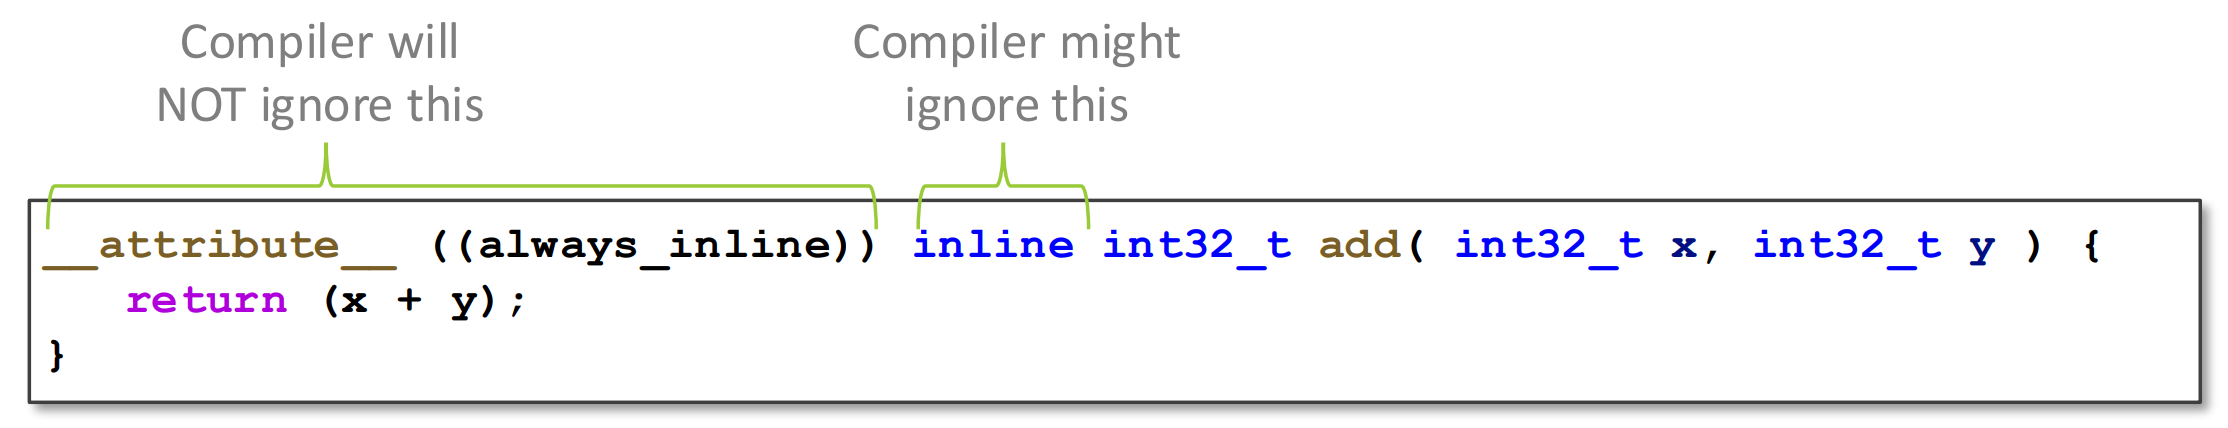
\includegraphics[width=0.75\linewidth]{img/image83.png}
\end{figure}


\subsection{Function Pragmas}

Pragmas are preprocessor directives that provide special instructions to the compiler via software and not
command line.

\begin{lstlisting}[language=c++]

    #pragma GCC push
    #pragma GCC optimize ("O0")
    int32_t add( int32_t x, int32_t y ){
        return (x + y);
    }
    #pragma GCC pop
\end{lstlisting}

\section{Preprocessor Directives}

\begin{figure}[H]
    \centering
    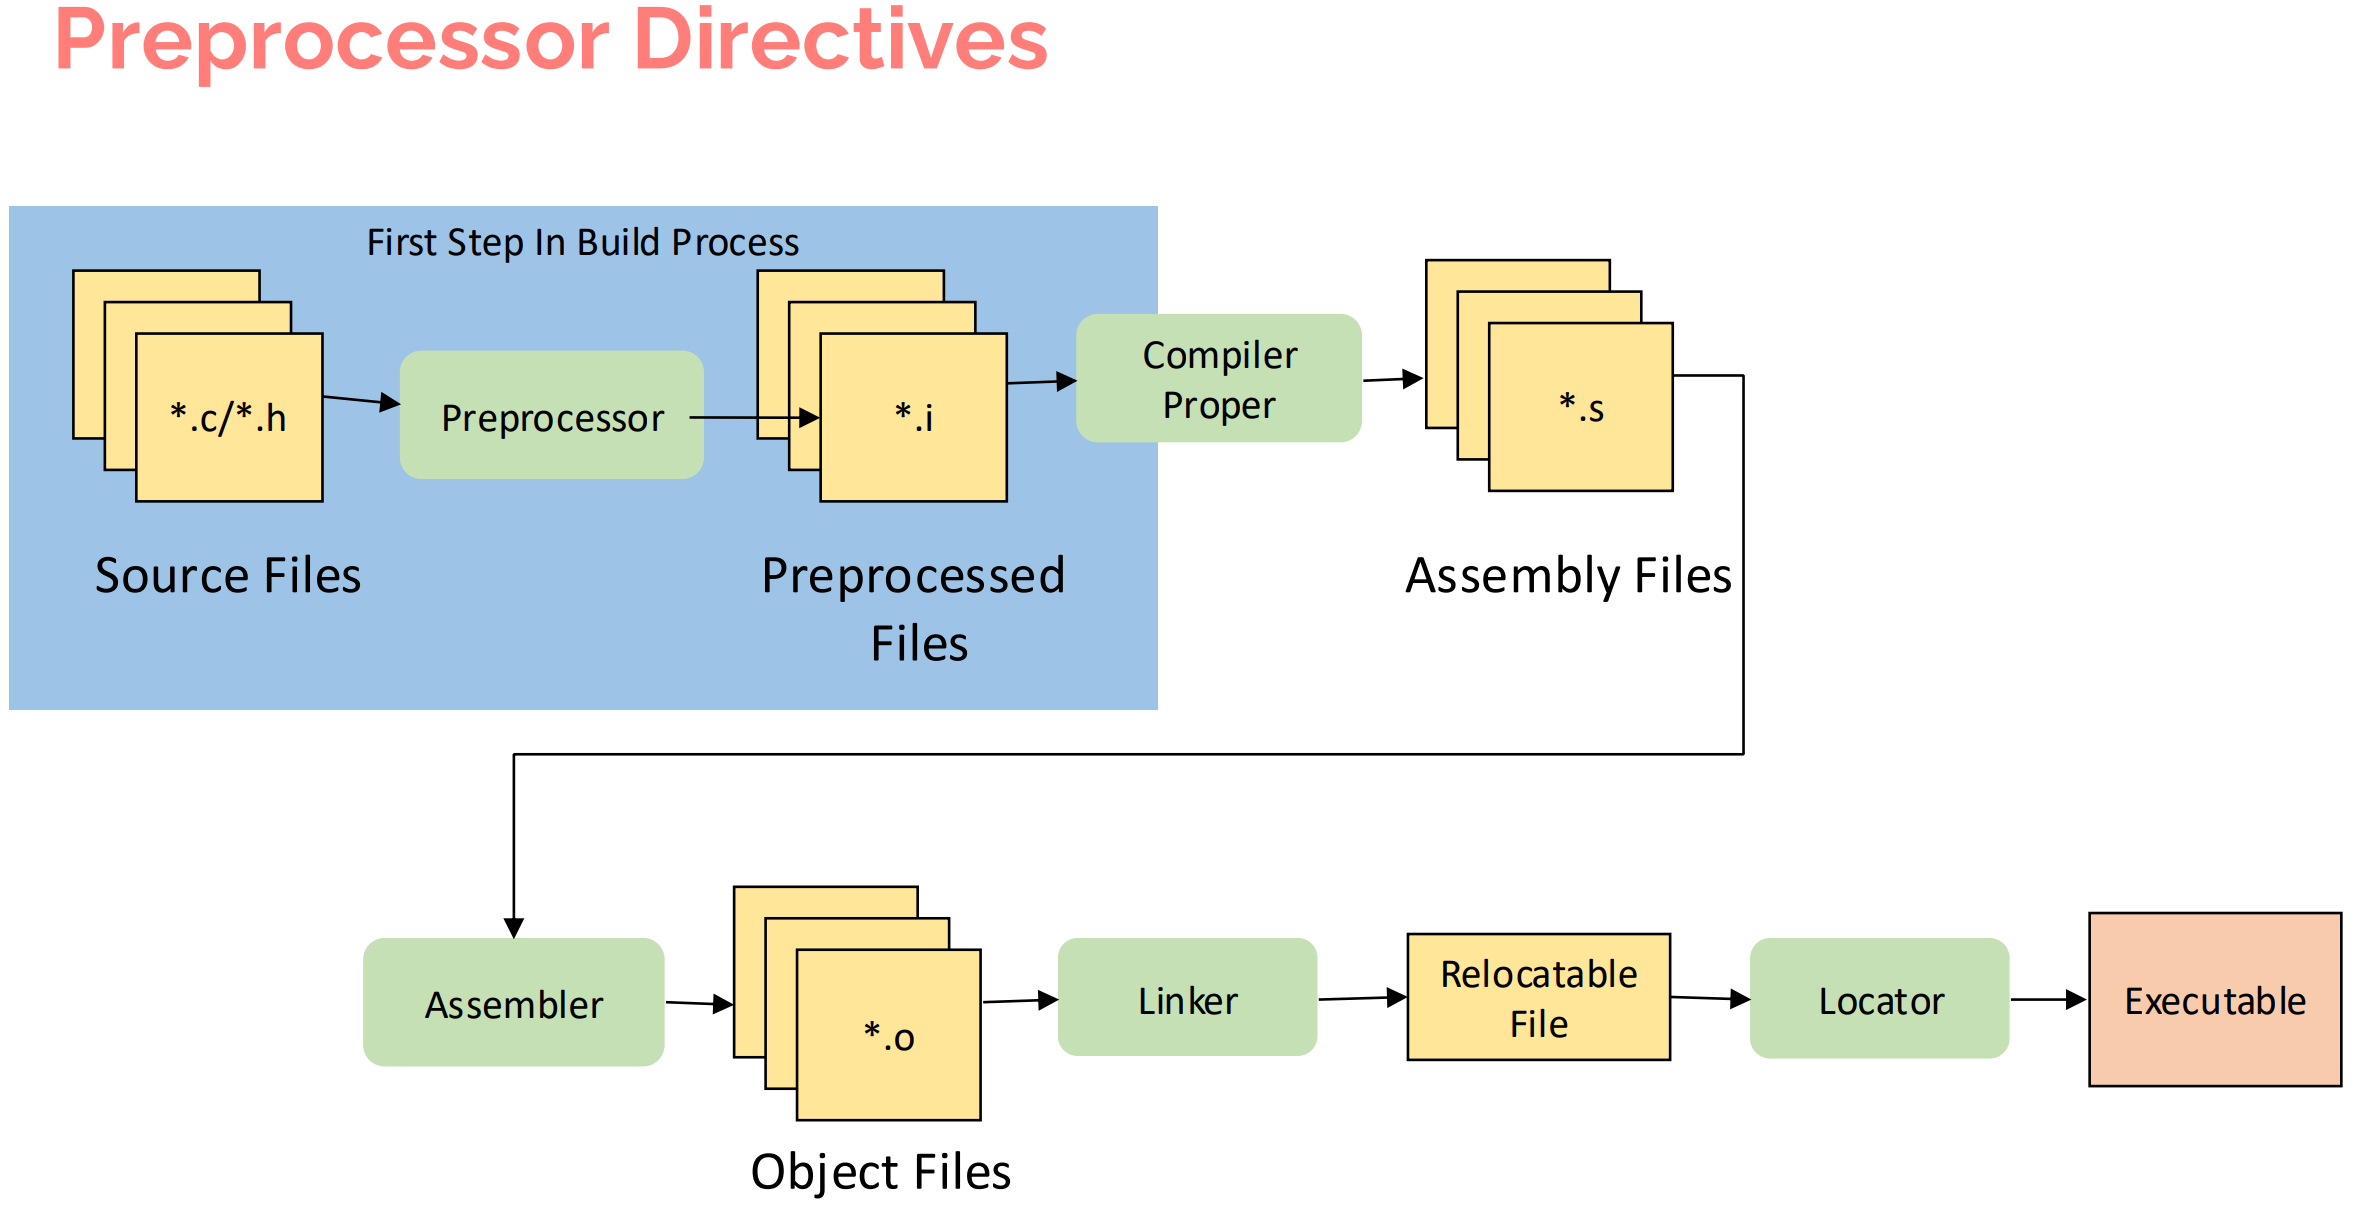
\includegraphics[width=0.75\linewidth]{img/image84.png}
\end{figure}

Preprocessor directives are special keywords used by the preprocessor before compilation.
All of them start with \# sign:

\begin{itemize}
    \item[--] Important Directives
    \item[--] \#define, \#undef
    \item[--] \#ifndef, \#ifdef, \#endif
    \item[--] \#include
    \item[--] \#warning, \#error
    \item[--] \#pragma
\end{itemize}


\begin{figure}[H]
    \centering
    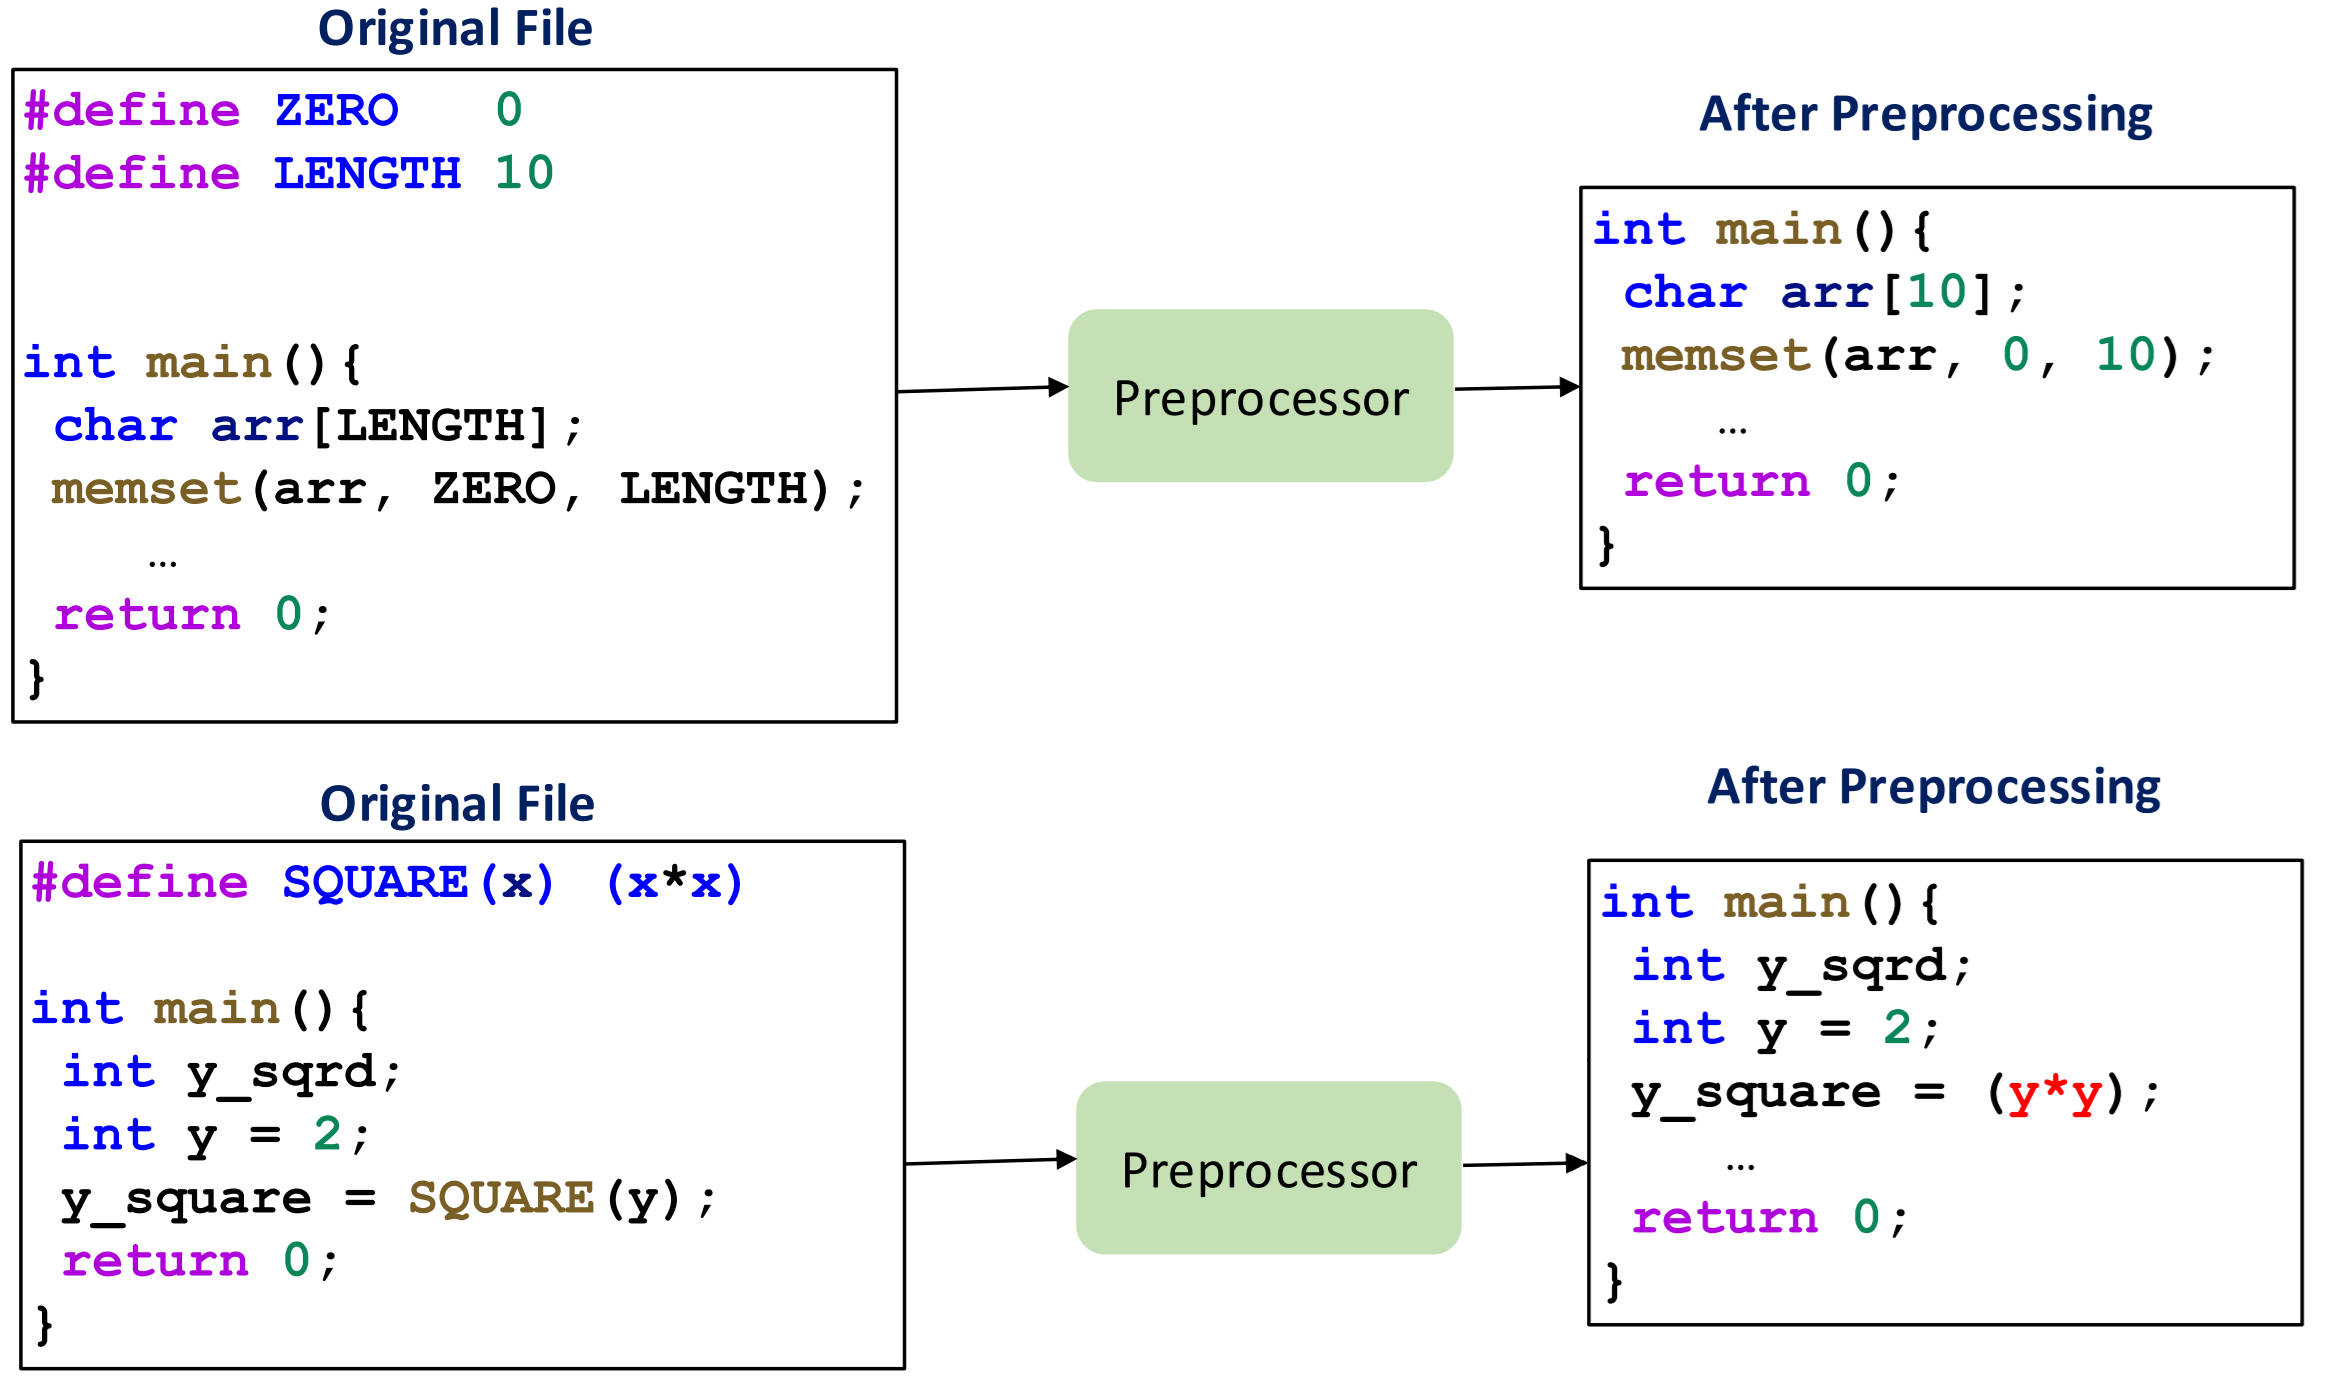
\includegraphics[width=0.75\linewidth]{img/image85.png}
\end{figure}

\paragraph{NOTE:} pay attention of undefined behavior (y++, it becames $2*3$).

\section{TI DriverLib}

The DriverLib is a software layer to the programmer: facilitates higher level of programming compared to direct register accesses

\begin{figure}[H]
    \centering
    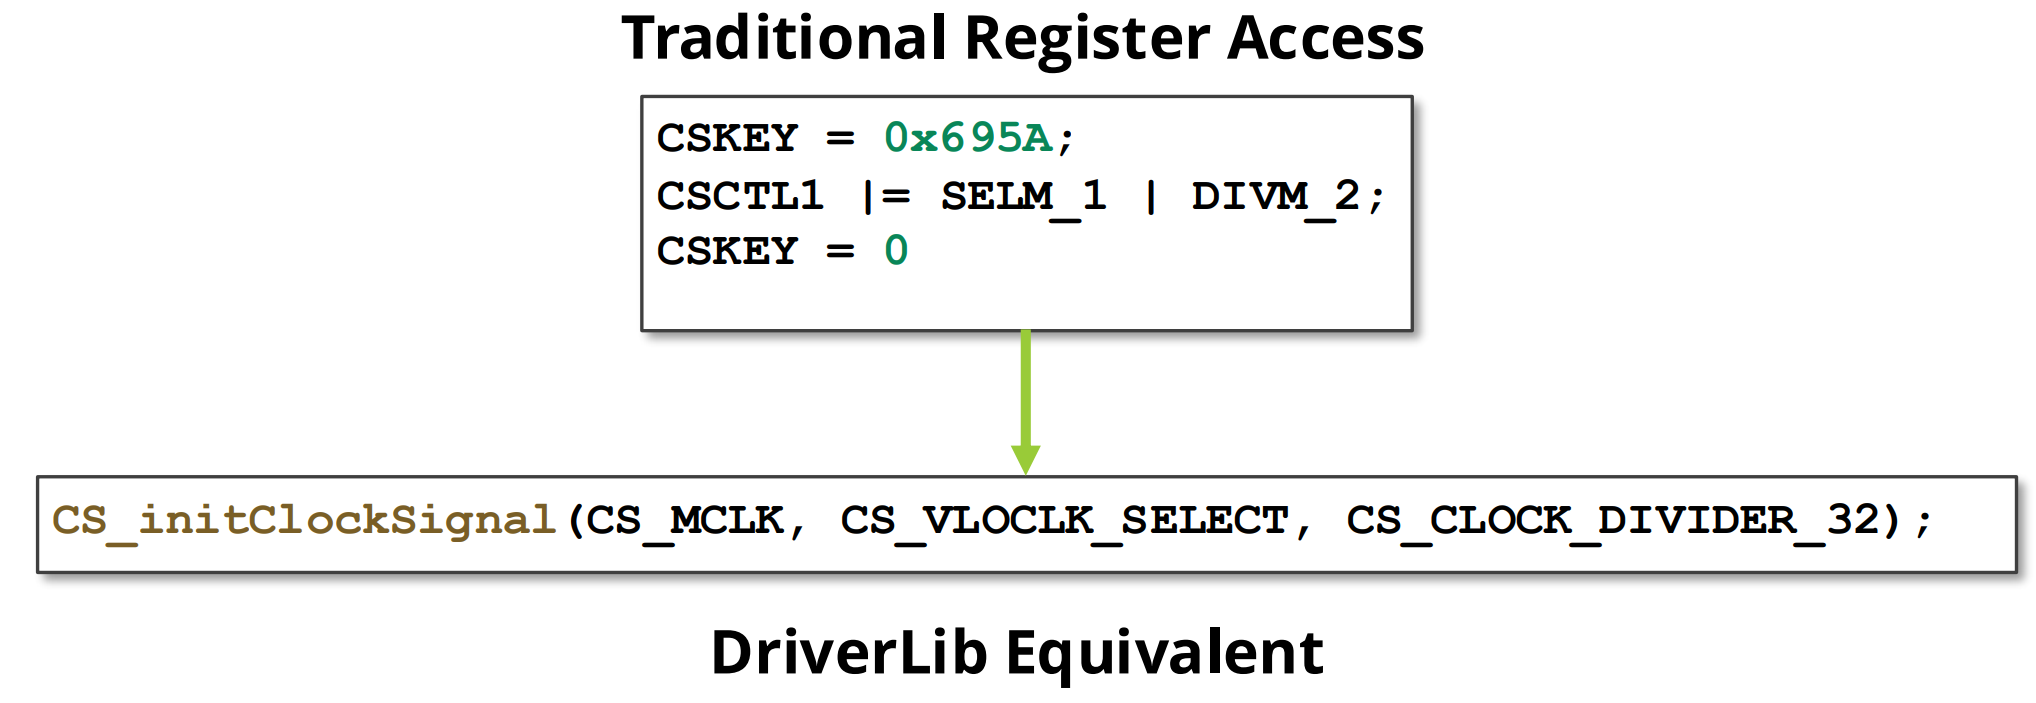
\includegraphics[width=0.75\linewidth]{img/image86.png}
\end{figure}